% QAOA circuit of notebook 45c, Eq. (9), drawn for MaxCut on the 4-vertex ring (edges 01, 12, 23, 30).
% |+>^N prepared by H on every qubit; layer l: U_C(gamma_l) = prod_edges exp(-i gamma_l Z_i Z_j) = prod R_ZZ(2 gamma_l),
% then U_B(beta_l) = prod_q R_x(2 beta_l); p layers; measurement in the computational basis gives a string z with cost C(z).
% Inset: Eq. (14), exp(-i theta Z_i Z_j) = CNOT_ij R_z(2 theta)_j CNOT_ij.  Right: the ring with an optimal cut.
\documentclass[tikz,border=6pt]{standalone}
\usepackage{amsmath,amssymb,bm}
\usetikzlibrary{arrows.meta,decorations.pathreplacing,calc,positioning}
\newcommand{\ket}[1]{\lvert #1\rangle}
\begin{document}
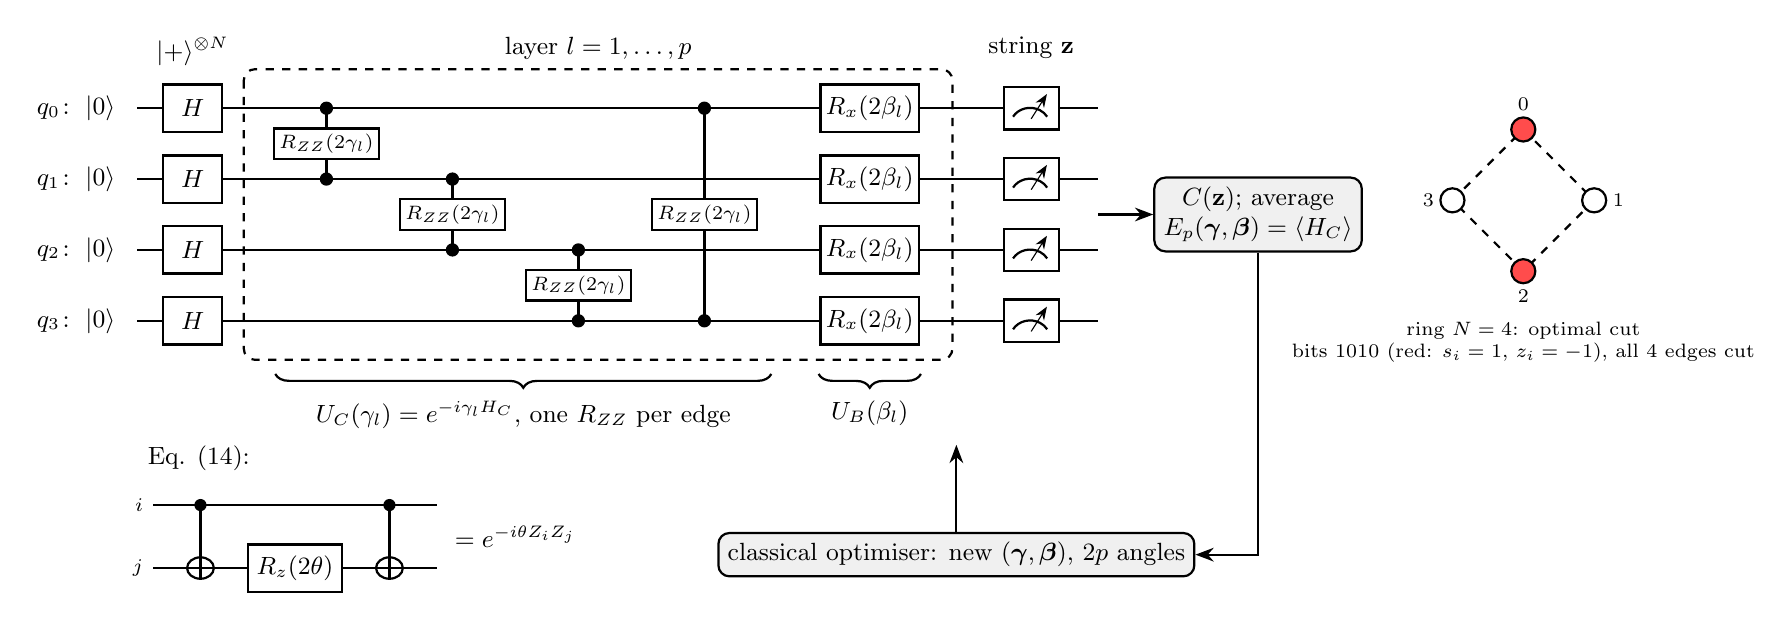
\begin{tikzpicture}[thick, >=Stealth, x=1cm, y=0.9cm,
    gate/.style={draw, fill=white, minimum height=0.6cm, minimum width=0.75cm, inner sep=2pt, font=\small},
    zz/.style={draw, fill=white, inner sep=2pt, font=\scriptsize}]
  % wires
  \foreach \q in {0,...,3} {
    \node[anchor=east, font=\small] at (-0.15,-\q) {$q_{\q}\!:\ \ket{0}$};
    \draw (0,-\q) -- (12.2,-\q);
  }
  % Hadamards
  \foreach \q in {0,...,3} \node[gate] at (0.7,-\q) {$H$};
  \node[font=\small] at (0.7,0.8) {$\ket{+}^{\otimes N}$};
  % layer box
  \draw[dashed, rounded corners] (1.35,0.55) rectangle (10.35,-3.55);
  \node[font=\small] at (5.85,0.85) {layer $l=1,\dots,p$};
  % cost layer: R_ZZ on the four edges, dot-line-dot with the angle on the line
  \newcommand{\zzgate}[3]{% x, q_i, q_j
    \fill (#1,-#2) circle (2.4pt); \fill (#1,-#3) circle (2.4pt);
    \draw (#1,-#2) -- (#1,-#3);
    \node[zz] at (#1,{-(#2+#3)/2}) {$R_{ZZ}(2\gamma_l)$};}
  \zzgate{2.4}{0}{1}
  \zzgate{4.0}{1}{2}
  \zzgate{5.6}{2}{3}
  \zzgate{7.2}{0}{3}
  \draw[decorate, decoration={brace, amplitude=5pt, mirror}] (1.75,-3.75) -- (8.05,-3.75)
       node[midway, below=6pt, font=\small] {$U_C(\gamma_l)=e^{-i\gamma_lH_C}$, one $R_{ZZ}$ per edge};
  % mixer
  \foreach \q in {0,...,3} \node[gate] at (9.3,-\q) {$R_x(2\beta_l)$};
  \draw[decorate, decoration={brace, amplitude=5pt, mirror}] (8.65,-3.75) -- (9.95,-3.75)
       node[midway, below=6pt, font=\small] {$U_B(\beta_l)$};
  % measurement
  \foreach \q in {0,...,3} {
    \draw[fill=white] (11.0,-\q+0.3) rectangle (11.7,-\q-0.3);
    \draw (11.12,-\q-0.12) arc (150:30:0.25);
    \draw[->, thin] (11.35,-\q-0.15) -- (11.55,-\q+0.2);
  }
  \node[font=\small, align=center] at (11.35,0.85) {string $\mathbf z$};
  \draw[->] (12.2,-1.5) -- (12.9,-1.5);
  \node[draw, rounded corners, fill=gray!12, font=\small, align=center, anchor=west] (cost) at (12.9,-1.5)
       {$C(\mathbf z)$; average\\ $E_p(\boldsymbol\gamma,\boldsymbol\beta)=\langle H_C\rangle$};
  % classical optimiser loop
  \node[draw, rounded corners, fill=gray!12, font=\small] (opt) at (10.4,-6.3)
       {classical optimiser: new $(\boldsymbol\gamma,\boldsymbol\beta)$, $2p$ angles};
  \draw[->] (cost.south) |- (opt.east);
  \draw[->] (opt.north) -- (opt.north |- 0,-4.75);
  % inset: compilation of R_ZZ, Eq. (14)
  \begin{scope}[shift={(0.2,-5.6)}, y=0.8cm]
    \node[anchor=west, font=\small] at (-0.2,0.75) {Eq. (14):};
    \draw (0,0) -- (3.6,0); \draw (0,-1) -- (3.6,-1);
    \node[font=\scriptsize, anchor=east] at (0,0) {$i$}; \node[font=\scriptsize, anchor=east] at (0,-1) {$j$};
    \fill (0.6,0) circle (2.2pt); \draw (0.6,0) -- (0.6,-1.17); \draw (0.6,-1) circle (0.17);
    \node[gate, minimum width=1.2cm] at (1.8,-1) {$R_z(2\theta)$};
    \fill (3.0,0) circle (2.2pt); \draw (3.0,0) -- (3.0,-1.17); \draw (3.0,-1) circle (0.17);
    \node[font=\small, anchor=west] at (3.7,-0.5) {$=e^{-i\theta Z_iZ_j}$};
  \end{scope}
  % graph: 4-ring with an optimal cut
  \begin{scope}[shift={(17.6,-1.3)}, x=0.9cm, y=0.9cm]
    \coordinate (v0) at (0,1); \coordinate (v1) at (1,0); \coordinate (v2) at (0,-1); \coordinate (v3) at (-1,0);
    \foreach \a/\b in {v0/v1, v1/v2, v2/v3, v3/v0} \draw[dashed] (\a) -- (\b);
    \foreach \v/\c in {v0/red!70, v2/red!70, v1/white, v3/white} \filldraw[fill=\c, draw=black] (\v) circle (0.17);
    \foreach \v/\n/\pos in {v0/0/above, v1/1/right, v2/2/below, v3/3/left} \node[font=\scriptsize, \pos=3pt] at (\v) {$\n$};
    \node[font=\scriptsize, align=center] at (0,-2.0) {ring $N=4$: optimal cut\\ bits $1010$ (red: $s_i=1$, $z_i=-1$), all 4 edges cut};
  \end{scope}
\end{tikzpicture}
\end{document}
